\begin{figure}[ht] 
 	\centering 
 	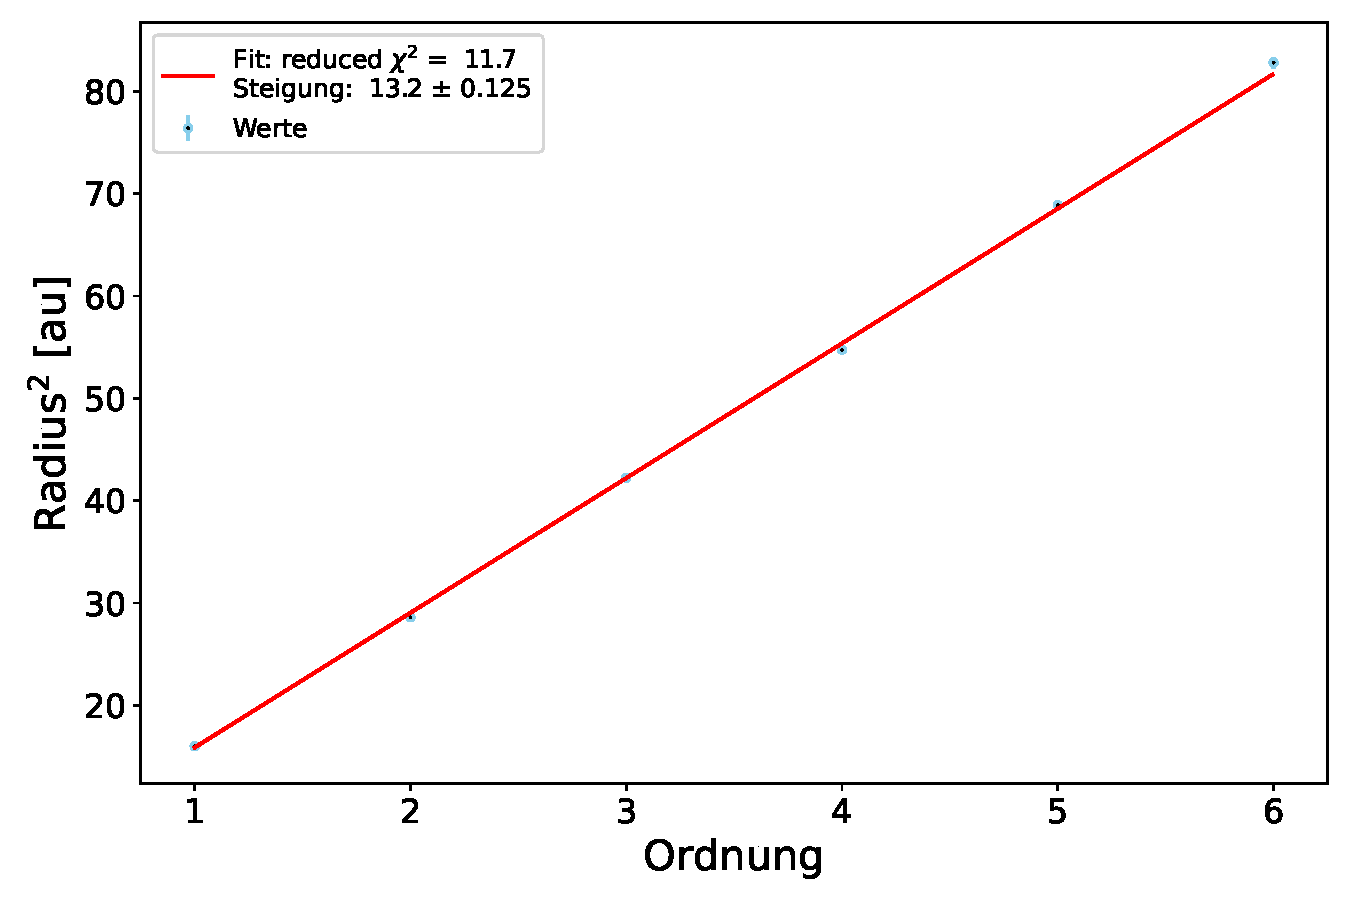
\includegraphics[width= 0.65 \textwidth]{Fits/messung3_Ring1_Tim_Fit.pdf} 
	\caption{messung3_Ring1_Tim, Fit} 
 	\label{fig:messung3_Ring1_Tim, Fit} 
\end{figure}
 \\ 
\begin{table}[ht] 
\centering 
\caption{messung3_Ring1_Tim, Fit Parameter Tabelle} 
\label{tab:my-table}
\begin{tabular}{|l|c|}
\hline
Parameter Name	&	Wert \\ \hline
slope	&	 13.166 \pm  0.125\\ \hline
intercept	&	 2.714 \pm  0.269\\ \hline
\end{tabular} 
\end{table}